%      Awab you idiot. WHy you do this
%      ps. hi person reading this (probs sukaina)

\documentclass{article}
\usepackage[utf8]{inputenc}
\usepackage[T1]{fontenc}
\usepackage{microtype}
\usepackage{graphicx}
\setlength{\parindent}{2pt}
%To get rid of indents cause miss amna hates them 
\usepackage{fancyhdr}
\usepackage{float}
\usepackage{lipsum}
\usepackage{newspaper}
%that's the one which makes the magic happen
\usepackage{newspaper-mod}
%%to redefine the headline and byline style if you want to.
%% These can be issued just before any
%% byline or headline in the paper, to
%% individually style each article
%%
% \renewcommand{\headlinestyle}{\itshape\Large\lsstyle}
% \renewcommand{\bylinestyle}{\bfseries\Large\raggedright}

\usepackage{multicol}
%For making columns using command \begin{multicols}{2}....\end{multicols}

%Fancy images
\usepackage{picinpar}
%uasage of picinpar:
%\begin{window}[1,l,\includegraphics{},caption]xxxxx\end{window}

% \begin{window}[2,r,\includegraphics[width=1.0in]{atom.jpg},\centerline{The Atom}] The \verb+multicol+ package allows using multiple columns without starting a new page.  Using floats is not possible in a columns environment, however with the \verb+picinpar+ package, I can set a picture inside a block of text---just like you one you see here.  Isn't \LaTeX{} cool?
% And now we're just filling more space, and yet more space.  
% \end{window}


% TODO: Change the font to Times New Roman



%Metadata you shouldn't change
\SetPaperName{
          %  
\includegraphics[scale=0.3]{fps}
        % \scalerel*{
\includegraphics{fps}}{f}
            FPS Eagles:   
         \hfill  
\includegraphics[height=\fontcharht\font`\B]{cfps} 
      }
\SetHeaderName{FPS Eagles}
\SetPaperLocation{
%    \centering
   %\begin{figure}
    %   \centering
  %  \vspace{5mm}
  %  
\includegraphics[scale=0.12]{lfps} 
   %  
\includegraphics[scale=0.09]{W}
   %\end{figure}
    
   
}
\SetPaperSlogan{
            %     
\includegraphics[scale=0.3]{fps}
                ``\textit{FPSonians are the best; second to none!}''
              %  
\includegraphics[scale=0.1]{cfps}
                }
\SetPaperPrice{By Awab Qureshi and Sukaina Kazmi; batch 2020}
\cfoot{\textit{FPSonians are the best; second to none!}}


% Metadata you should change
\date{\today}
\currentvolume{1}
\currentissue{1}




\begin{document}
\maketitle
\large 

%The beginning 

%                               FRONT PAGE

\headline{PLASTIC}\textbf{by Awab Ahmed Qureshi XI-D}

Researchers recently probed fish-life in the deepest parts of our ocean and found something shocking. In their digestive tracts were quantities of microplastics. The study raised several concerns. Finding microplastics at such a depth means that even the deepest parts of our oceans are not safe from our litter.More and more plastic is thrown into our oceans every day with some estimates ranging between 4.8~12.7 million tonnes per Annum.\newline Indeed microplastics are quite dangerous as the ones found in such fish could easily transfer up the food chain and into our food supply, causing a plethora of adverse health effects.

Students in the SLC in FPS realised this crisis, and thus, to prevent it, worked with the admin to ban the sale of all plastic bottles in the canteen. The ban, which was put in place earlier this term has reduced the plastic bottle waste OLDC generates to \boldsymbol{0}. In place of this, students can now refill their bottles at a lower rate from the canteen's water filter.

It is hoped that our contribution, whilst small, will make a difference by discouraging the use of disposable plastics and will a step on the long road towards a green future. 


\closearticle
%do \closearticle for that double line bar

\begin{multicols}{2}
%to make columns

\headline{Escape to Wonderland}\textbf{by Sukaina Kazmi XI-C}

Friday 11th October was a night to remember for all grade 11s. FPS A-Levels had held its 4th annual “Escape to Wonderland” which unfortunately the last of its kind. The activity aided in enhancing and bringing out a student’s team building and problem solving skills as the students hurriedly pieced together multiple clues and puzzles to save the world from the apocalypse .Students in teams of eight were locked in a military bunker with an attendant and had approximately an hour to stop the virus from spreading into the atmosphere and escaping the room. Students had to channel their cognitive skills to scavenge the keys to the buzzer thereby emerging triumphant. Once the students succeeded in escaping the room they gained entry to the magical wonderland full of food, games, rides and music for them to dance the night away. The night ended up being a truly memorable event which I’m sure this batch is to remember.


\headline{FPS Ignite}\textbf{by Laiba Abid XI-C}

Ignite is an annual three day entrepreneurial event hosted by FPS A Levels and provides students a platform to test out their entrepreneurial ideas. Participants form 4-member delegations and the shortlisted ones then partake in bidding for their desired industry. Upon receiving the bidding results, they then design a pitch presentation, and legal documents for their product. 

On the first day delegations were tasked with designing billboards. On the second day they raced to solve a crisis and shoot their TV commercial. In the evening, participants got to socialize with their batch-mates and blow off some steam in the Social. The third day kept everyone on their toes as the delegations had to go through a ‘surprise round’, pitch their product to the investors and present their tvc and billboard. The event ended with a grand award ceremony where various trophies were given out.

\end{multicols}
\pagebreak 
%to make sure stuff stays on this page

%                              2ND PAGE 

\headline{Our Lack of Awareness}\textbf{by Arham Siddiqui XI-B}

The lack of awareness on gender rights, hygiene, citizen rights etc. is unfortunately an issue Pakistan struggles with. Even worse is the realization that millions of people in rural and urban settings are not aware of how they should be treated by the people around them, by their rightful authorities or even how they should treat their own selves. 

Whilst being a fact more commonly widespread nowadays, female oppression in workplaces and in their personal lives is still a big issue. Millions of Pakistani women forcefully succumb to fulfilling their stigmatised role in society instead of their aspirations because they are not educated on their rights as a woman. This lack of awareness creates more problems for females in different walks of life.

Another instance where lack of awareness hinders Pakistani society is in hygiene, which has caused a highly escalating infant mortality rate. This problem is further exacerbated in rural areas of the country, where sanitary methods of keeping newborns clean and healthy during their weaning phase is a null prospect. No proper post-natal care is propagated, which results in thousands of kids failing to reach the age of 5. 

The people of Pakistan have also never been made fully aware of the democratic rights they possess, which has led to Pakistan wading in turbulent waters. Many citizens far and wide remain complacent, not willing to put in the effort of exercising their voice by casting a vote. When faced with sights of social injustice the people shrug it off as something that cannot be changed. This has not only made the common man more uninterested in local affairs, but has also led to the country sinking into a state of regression. It is no secret that democracies fail when citizens become disinterested. 

A viable approach to all this is education. Together, as a single person or neighbourhood - with or without the government - we can spread awareness of our rights. Fortunately change has already begun. As the social movements in recent years have shown, the young populace is becoming acutely aware of their rights. May this create a better society for us all.


\closearticle

\begin{multicols}{2}
\headline{Sports}


Sarah Sajjad is an ambitious champion who represents in the National Olympic Games held in Peshawar, and has impressed us once again as the youngest throwball athlete of the event. This is not the first time Sara has made FPS proud as the outstanding athletic virtuoso also made us all proud last year in inter-school competitions. 

She left for Peshawar, along with her mother for the nerve wrecking journey, on Nov. 8th. The team started their first match with Balochistan, winning it with a lead of 20 points. Among the 6 games that were held: two qualifying matches, two semi-finals and two finals; Sindh won all 6 of them. Sara honored us all, as well as her family, and most importantly her parents, with her trophy and gold medal.  


%\end{multicols}
\closearticle
%\begin{multicols}{2}

\headline{This Week in History}
1912-The ocean liner Titanic sinks after hitting an iceberg in the North Atlantic Sea.

1966-Football’s World Cup is stolen from a display in London. A dog finds it a week later, under a hedge.

1968-The funeral of Martin Luther King Jr. takes place.

1973-The art world mourns Spanish artist Pablo Picasso who dies in France aged 91.
\closearticle

\headline{Upcoming Events}
THE WINTER FEST ~ 19th December 2019
\closearticle
\end{multicols}

\pagebreak


%                               3RD PAGE

\headline{What's Up With Tech?}
\begin{multicols}{2}
    \headline{Sony Announces PS5}
We have been waiting to find out about the PS4's replacement for a while now, but details have been kept under wraps. That is, until now, because Sony has just released information.

The new console will include a high-speed solid-state hard drive (SSD) to lessen game load times, 3D audio, and will support ray-tracing graphics making your games look more realistic.

Sony is expected to release the PS5 (if it is even called that) late next year. Until then we'll have to wait and see what other information they release.
%\closearticle


\headline{Half-Life: Alyx}
    Valve has announced a new Half-Life game in over a decade. The news shocked fans, who thought they'd never see another installment in the series again. Many memes were popularised as fans grew restless such as the famous "Half-Life 3 confirmed" and "Valve can't count to 3".
    
    The game will be entirely in Virtual Reality, causing many to hope that it will bring VR headsets to general consumer's homes and pave the way for a new era. 
    
    Half-Life: Alyx releases in March next year and is likely to generate more hype and possibly break the internet at release.

%\vfill
%\closearticle

\end{multicols}
\closearticle

\begin{center}
\headline{Jokes, and Memes}

\includegraphics[height=5.5cm]{m1.jpeg}

\includegraphics[height=5.5cm]{m2.jpeg}

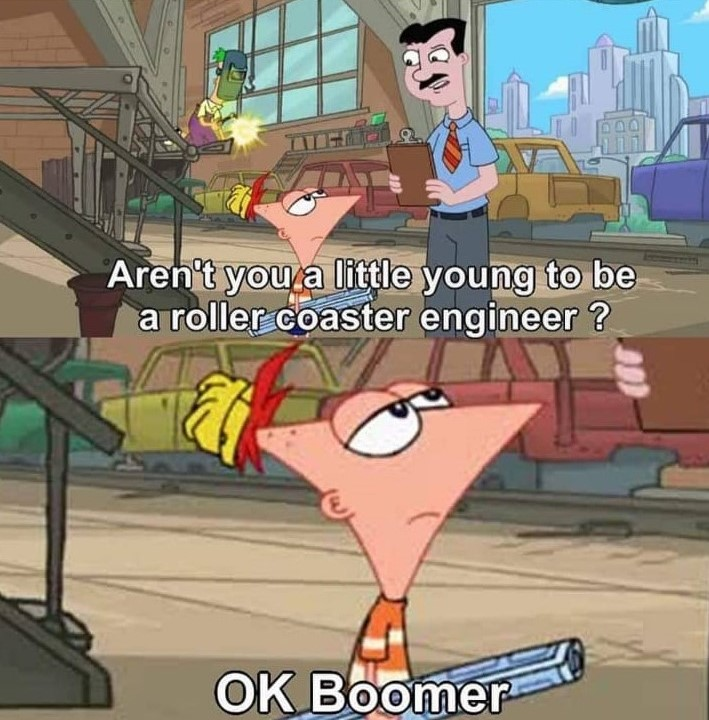
\includegraphics[height=6cm]{m3.jpeg}

\includegraphics[height=6cm]{m4.jpeg}
\end{center}

\pagebreak


%                            4TH PAGE

\begin{multicols}{2}

\headline{What about the Grammy's?}
The Grammy’s were entangled in controversy in 2018, after only one women, Alessia Cara, won an award. Asked to respond to the lack of female representation, Recording Academy president Neil Portnow said women needed "to step up." His comments sparked an outrage, and this year’s ceremony rang the changes, with Kacey Musgrave’s space-age country album Golden Hour taking home the main prize, presented by a new female host, Alicia Keys. As she picked up the best new artist trophy, British star Dua Lipa drove home the point, saying:” I guess this year we really stepped up.” Now two years later women are dominating the 2020 nominations. We’ll discover who wins when the 62nd annual Grammy Awards takes place on Sunday, 26th January 2020, hosted again by Alicia Keys.

\pagebreak


\end{multicols}

\end{document}
